\section{Results and Discussion}

\subsection{Temperature Distribution}

Figure~\ref{fig:contours} compares the numerical solution obtained using the finite-volume solver with the analytical solution of the Laplace equation. The two temperature fields exhibit excellent agreement throughout the computational domain. The smooth variation of the temperature contours and the close correspondence between the numerical and analytical solutions demonstrate that the governing equation, spatial discretization, and boundary-condition implementation have been correctly incorporated into the solver.

\begin{figure}[H]
    \centering
    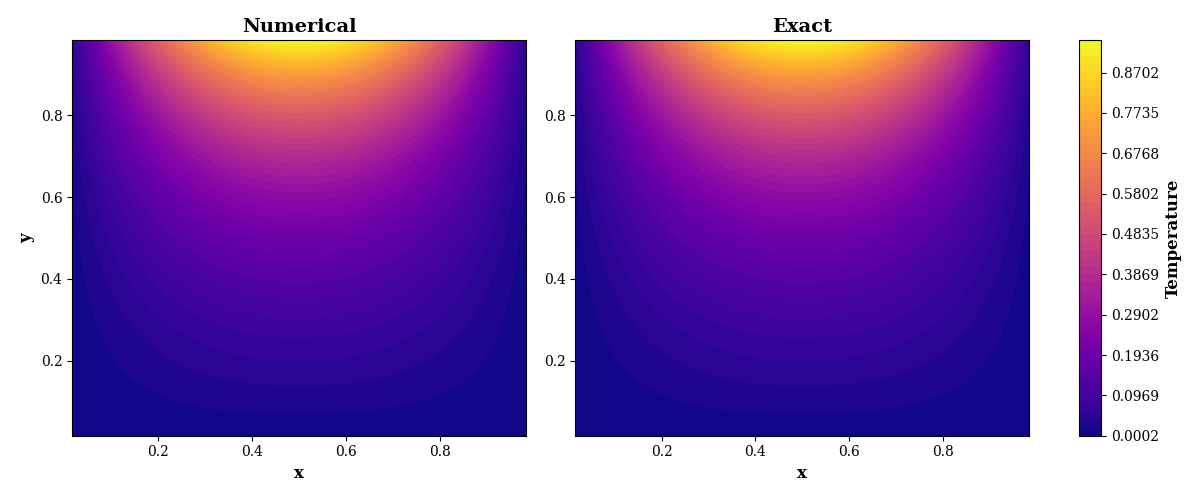
\includegraphics[width=\textwidth]{figures/temperature_contours.png}
    \caption{Comparison of the numerical and analytical temperature distributions.}
    \label{fig:contours}
\end{figure}

%%%%%%%%%%%%%%%%%%%%%%%%%%%%%%%%%%%%%%%%%%%%%%%%%%%%%%%%%%%%%

\subsection{Error Field}

To quantify the numerical accuracy, the pointwise error field was computed as the difference between the analytical and numerical temperature distributions. The resulting error field is shown in Figure~\ref{fig:error}.

The error remains small throughout the computational domain, confirming the second-order accuracy of the spatial discretization. The largest errors occur in regions of relatively large temperature gradients, which is consistent with the expected behavior of finite-volume discretizations on a finite-resolution mesh.

\begin{figure}[H]
    \centering
    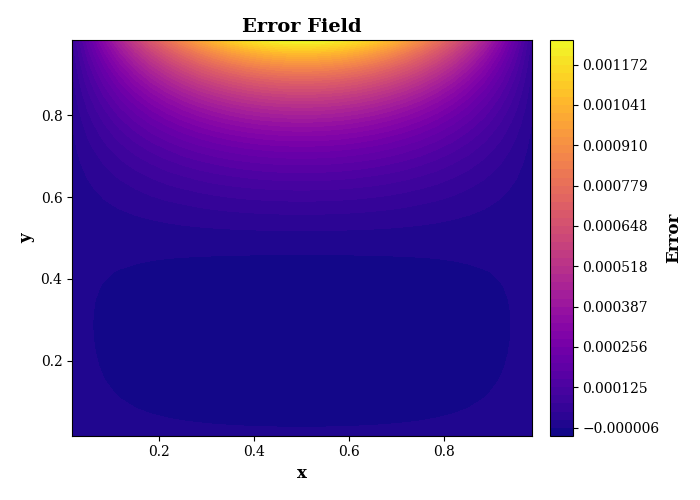
\includegraphics[width=0.65\textwidth]{figures/error_field.png}
    \caption{Spatial distribution of the numerical error.}
    \label{fig:error}
\end{figure}

%%%%%%%%%%%%%%%%%%%%%%%%%%%%%%%%%%%%%%%%%%%%%%%%%%%%%%%%%%%%%

\subsection{Convergence History}

The convergence behavior of the Point Gauss-Seidel solver was monitored using the $L_2$ residual norm. Figure~\ref{fig:residual} presents the residual history as functions of both iteration number and computation time.

The residual decreases monotonically until the prescribed convergence tolerance is satisfied, indicating stable convergence of the iterative solution procedure. The residual-time history additionally provides a useful measure of computational performance and establishes a baseline for future comparisons with accelerated iterative methods such as Successive Over-Relaxation (SOR), Line Gauss-Seidel, ADI, and multigrid methods.

\begin{figure}[H]
    \centering
    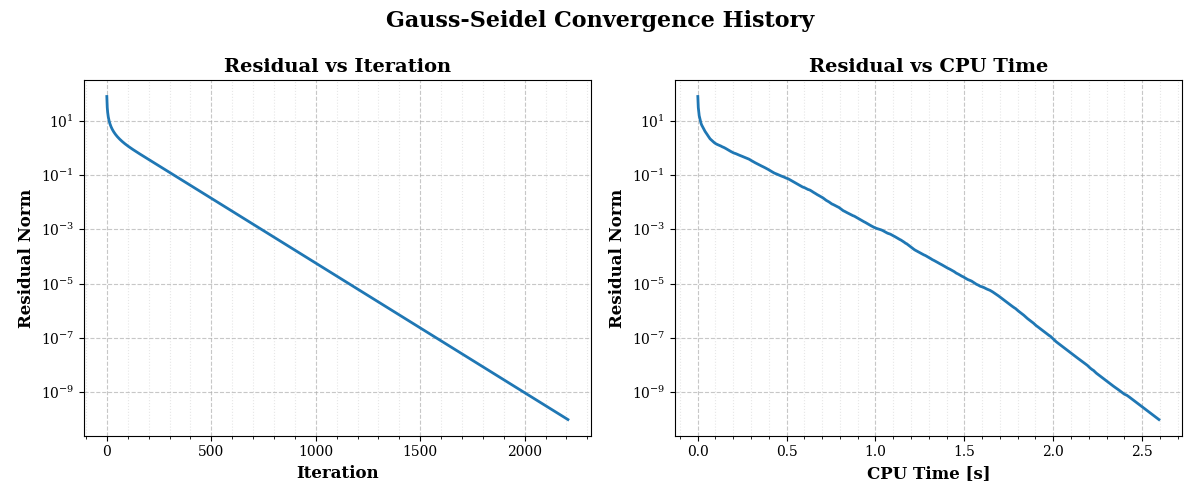
\includegraphics[width=\textwidth]{figures/residual_history.png}
    \caption{Residual convergence histories with respect to iteration count and computation time.}
    \label{fig:residual}
\end{figure}

%%%%%%%%%%%%%%%%%%%%%%%%%%%%%%%%%%%%%%%%%%%%%%%%%%%%%%%%%%%%%

\subsection{Line-Cut Comparison}

To further verify the numerical implementation, horizontal and vertical line cuts were extracted at several locations within the computational domain and compared with the corresponding analytical solution.

As shown in Figure~\ref{fig:linecuts}, the numerical and analytical profiles are nearly indistinguishable for all selected cut locations. The close agreement demonstrates that the solver accurately reproduces both the magnitude and spatial variation of the analytical temperature field.

\begin{figure}[H]
    \centering
    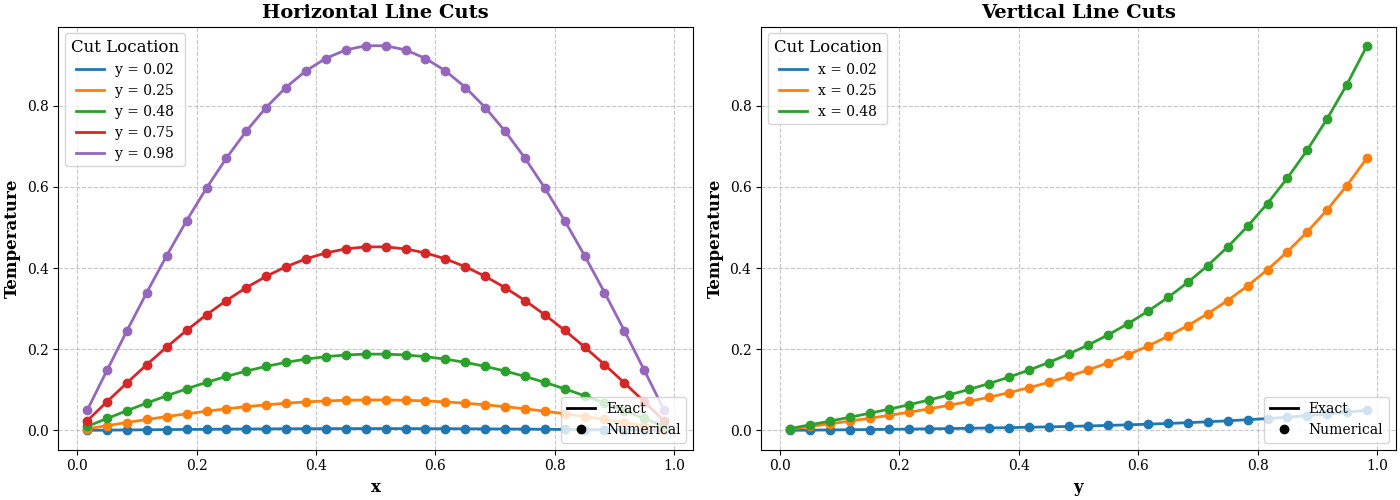
\includegraphics[width=\textwidth]{figures/line_cuts.png}
    \caption{Comparison of numerical and analytical temperature profiles along selected horizontal and vertical line cuts.}
    \label{fig:linecuts}
\end{figure}